\subchapter{Drzewa}

\exercise %B.5-1
Rys.\ \ref{fig:B.5-1} ilustruje wszystkie szukane drzewa.
\begin{figure}[!ht]
	\centering \begin{tikzpicture}[
	outer/.append style = {node distance=15mm and 12mm},
	inner/.style = {draw=none, fill=none, node distance=3.5mm, every node/.style=tree node},
	level/.append style = {sibling distance=30mm/2^#1}
]

\node[outer] (pic a) {
\begin{tikzpicture}
	\node[inner] (pic a1) {
	\begin{tikzpicture}[anchor=center]
		\node {$A$}
			child {node {$B$}
				child {node {$C$}}
			};
	\end{tikzpicture}
	};
	\node[inner, right=of pic a1] (pic a2) {
	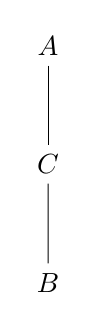
\begin{tikzpicture}[anchor=center]
		\node {$A$}
			child {node {$C$}
				child {node {$B$}}
			};
	\end{tikzpicture}
	};
	\node[inner, right=of pic a2] {
	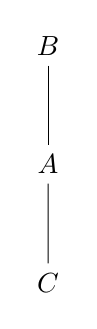
\begin{tikzpicture}[anchor=center]
		\node {$B$}
			child {node {$A$}
				child {node {$C$}}
			};
	\end{tikzpicture}
	};
\end{tikzpicture}
};

\node[outer, right=of pic a] (pic b) {
\begin{tikzpicture}
	\node[inner] (pic b1) {
	\begin{tikzpicture}[anchor=center]
		\node {$A$}
			child {node {$B$}
				child {node {$C$}}
			};
	\end{tikzpicture}
	};
	\node[inner, right=of pic b1] (pic b2) {
	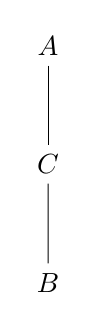
\begin{tikzpicture}[anchor=center]
		\node {$A$}
			child {node {$C$}
				child {node {$B$}}
			};
	\end{tikzpicture}
	};
	\node[inner, right=of pic b2.north east, anchor=north west] {
	\begin{tikzpicture}[anchor=center]
		\node {$A$}
			child {node {$B$}}
			child {node {$C$}};
	\end{tikzpicture}
	};
\end{tikzpicture}
};

\node[outer, right=of pic b] (pic c) {
\begin{tikzpicture}
	\node[inner] (pic c1) {
	\begin{tikzpicture}[anchor=center]
		\node {$A$}
			child {node {$B$}
				child {node {$C$}}
			};
	\end{tikzpicture}
	};
	\node[inner, right=of pic c1] (pic c2) {
	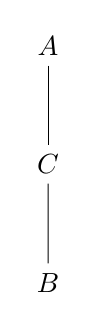
\begin{tikzpicture}[anchor=center]
		\node {$A$}
			child {node {$C$}
				child {node {$B$}}
			};
	\end{tikzpicture}
	};
	\node[inner, right=of pic c2.north east, anchor=north west] (pic c3) {
	\begin{tikzpicture}[anchor=center]
		\node {$A$}
			child {node {$B$}}
			child {node {$C$}};
	\end{tikzpicture}
	};
	\node[inner, right=of pic c3.north east, anchor=north west] {
	\begin{tikzpicture}[anchor=center]
		\node {$A$}
			child {node {$C$}}
			child {node {$B$}};
	\end{tikzpicture}
	};
\end{tikzpicture}
};

\node[draw=none, fill=none] (bottom center) at ($ (pic a.south west)!.5!(pic c.south east) $) {};

\node[outer, below=of bottom center, anchor=north] (pic d) {
\begin{tikzpicture}
	\node[inner] (pic d1) {
	\begin{tikzpicture}[anchor=center]
		\node {$A$}
			child[missing]
			child {node {$B$}
				child[missing]
				child {node {$C$}}
			};
	\end{tikzpicture}
	};
	\node[inner, right=of pic d1] (pic d2) {
	\begin{tikzpicture}[anchor=center]
		\node {$A$}
			child[missing]
			child {node {$B$}
				child {node {$C$}}
				child[missing]
			};
	\end{tikzpicture}
	};
	\node[inner, right=5mm of pic d2.north east, anchor=north west] (pic d3) {
	\begin{tikzpicture}[anchor=center]
		\node {$A$}
			child {node {$B$}}
			child {node {$C$}};
	\end{tikzpicture}
	};
	\node[inner, right=5mm of pic d3.north east, anchor=north west] (pic d4) {
	\begin{tikzpicture}[anchor=center]
		\node {$A$}
			child {node {$B$}
				child[missing]
				child {node {$C$}}
			}
			child[missing];
	\end{tikzpicture}
	};
	\node[inner, right=of pic d4] (pic d5) {
	\begin{tikzpicture}[anchor=center]
		\node {$A$}
			child {node {$B$}
				child {node {$C$}}
				child[missing]
			}
			child[missing];
	\end{tikzpicture}
	};
	\node[inner, below=of pic d1] (pic d6) {
	\begin{tikzpicture}[anchor=center]
		\node {$A$}
			child[missing]
			child {node {$C$}
				child[missing]
				child {node {$B$}}
			};
	\end{tikzpicture}
	};
	\node[inner, right=of pic d6] (pic d7) {
	\begin{tikzpicture}[anchor=center]
		\node {$A$}
			child[missing]
			child {node {$C$}
				child {node {$B$}}
				child[missing]
			};
	\end{tikzpicture}
	};
	\node[inner, right=5mm of pic d7.north east, anchor=north west] (pic d8) {
	\begin{tikzpicture}[anchor=center]
		\node {$A$}
			child {node {$C$}}
			child {node {$B$}};
	\end{tikzpicture}
	};
	\node[inner, right=5mm of pic d8.north east, anchor=north west] (pic d9) {
	\begin{tikzpicture}[anchor=center]
		\node {$A$}
			child {node {$C$}
				child[missing]
				child {node {$B$}}
			}
			child[missing];
	\end{tikzpicture}
	};
	\node[inner, right=of pic d9] {
	\begin{tikzpicture}[anchor=center]
		\node {$A$}
			child {node {$C$}
				child {node {$B$}}
				child[missing]
			}
			child[missing];
	\end{tikzpicture}
	};
\end{tikzpicture}
};

\foreach \x in {a,b,c,d} {
	\node[subpicture label, below=2mm of pic \x] {(\x)};
}

\end{tikzpicture}
	\caption{{\sffamily\bfseries(a)} Drzewa wolne o~3 wierzchołkach $A$, $B$ i~$C$.
{\sffamily\bfseries(b)} Drzewa ukorzenione o~węzłach $A$, $B$ i~$C$, w~których $A$ jest korzeniem.
{\sffamily\bfseries(c)} Drzewa uporządkowane o~węzłach $A$, $B$ i~$C$, w~których $A$ jest korzeniem.
{\sffamily\bfseries(d)} Drzewa binarne o~węzłach $A$, $B$ i~$C$, w~których $A$ jest korzeniem.} \label{fig:B.5-1}
\end{figure}

\exercise %B.5-2
Przypuśćmy, że twierdzenie jest fałszywe, czyli że wersja nieskierowana grafu $G$ nie tworzy drzewa, a~więc posiada cykl, w~szczególności cykl prosty (\refExercise{B.4-2}).
Niech $\langle v_1,v_2,\dots,v_k,v_1\rangle$ będzie takim cyklem.
Graf $G$ jest acykliczny, zatem dla pewnego $1\le l\le k$ istnieją krawędzie $\langle v_l,v_{l+1}\rangle$, $\langle v_{l+2},v_{l+1}\rangle\in E$, przy czym $v_{k+1}$ utożsamiamy z~$v_1$, a~$v_{k+2}$ z~$v_2$.
Wiemy z~założenia, że $v_0\leadsto v_l$ oraz $v_0\leadsto v_{l+2}$, zatem istnieją dwie różne ścieżki z~$v_0$ do $v_{l+1}$:
\[
	\langle v_0,\dots,v_l,v_{l+1}\rangle \quad\text{oraz}\quad \langle v_0,\dots,v_{l+2},v_{l+1}\rangle.
\]
Otrzymana sprzeczność prowadzi do wniosku, że wersja nieskierowana grafu $G$ jest acykliczna, zatem istotnie stanowi drzewo.

\exercise %B.5-3
Oznaczmy przez $n$, $n_0$, $n_2$, odpowiednio, całkowitą liczbę węzłów niepustego drzewa binarnego, liczbę jego liści oraz liczbę jego węzłów stopnia 2.
Jeśli $n=1$, to drzewo składa się tylko z~korzenia -- mamy więc $n_0=1$, $n_2=0$ i~$n_2=n_0-1$.

Załóżmy, że zależność $n_2=n_0-1$ jest prawdziwa dla dowolnego drzewa binarnego o~rozmiarze $n\ge1$.
Wstawmy do takiego drzewa nowy węzeł jako dodatkowy liść i~rozważmy powstałe drzewo o~rozmiarze $n'=n+1$.
Jeśli nowy węzeł został przyłączony do liścia oryginalnego drzewa, to liczba węzłów stopnia 2 w~nowym drzewie wynosi $n_2'=n_2$, a~liczba liści wynosi $n_0'=n_0$ i~oczywiście zależność $n_2'=n_0'-1$ pozostaje spełniona.
W~przeciwnym razie nowy węzeł został przyłączony do węzła o~stopniu 1.
Wtedy $n_2'=n_2+1$, $n_0'=n_0+1$ i~tu także zachodzi $n_2'=n_0'-1$.

\exercise %B.5-4
Udowodnimy nierówność $h\ge\lfloor\lg n\rfloor$ przez indukcję względem $n$.
Jeśli $n=1$, to drzewo posiada tylko jeden węzeł, więc $h=0$ i~nierówność oczywiście zachodzi.
Załóżmy teraz, że $n\ge2$ oraz że nierówność jest spełniona dla wszystkich drzew binarnych o~$n-1$ węzłach i~wysokości $h$.
Niech $T$ będzie jednym z~nich.
Dodając do niego nowy węzeł, tworzymy nowe drzewo $T'$ o~wysokości $h'$.
Rozważmy dwa przypadki w~zależności od położenia tego węzła w~drzewie $T'$.

Przyjmijmy najpierw, że nowy węzeł został umieszczony na co najwyżej \singledash{$h$}{tym} poziomie.
Wówczas $h'=h$.
Jedyny przypadek, gdy nierówność $h'\ge\lfloor\lg n\rfloor$ nie jest spełniona, występuje wówczas, gdy $n=2^{h+1}$, czyli gdy $T$ jest pełnym drzewem binarnym.
Ale każdy poziom takiego drzewa ma komplet węzłów, dlatego nowy węzeł może zostać umieszczony jedynie na \singledash{$(h+1)$}{szym} poziomie, co przeczy założeniu.
A~zatem nierówność jest spełniona.

W~przypadku, gdy nowy węzeł zajął w~$T'$ poziom $h+1$, jest $h'=h+1$.
Z~założenia indukcyjnego mamy $h\ge\lfloor\lg(n-1)\rfloor$, zatem wystarczy pokazać, że $\lfloor\lg(n-1)\rfloor+1\ge\lfloor\lg n\rfloor$.
Zauważmy, że dla dowolnej liczby rzeczywistej $x$ i~dowolnej liczby całkowitej $k$ zachodzi $\lfloor x\rfloor+k=\lfloor x+k\rfloor$.
Mamy więc
\[
    \lfloor\lg(n-1)\rfloor+1 = \lfloor\lg(n-1)+1\rfloor = \lfloor\lg(n-1)+\lg2\rfloor = \lfloor\lg(2n-2)\rfloor.
\]
Podłoga oraz logarytm przy podstawie 2 są funkcjami niemalejącymi, a~więc $\lfloor\lg(2n-2)\rfloor\ge\lfloor\lg n\rfloor$, o~ile $2n-2\ge n$, czyli gdy $n\ge2$.
Nierówność zachodzi zatem dla dowolnego drzewa binarnego.

\exercise %B.5-5
Dowodzimy przez indukcję względem $n$.
Gdy $n=0$, to drzewo jest puste, więc $i=e=0$ i~baza zachodzi.
Załóżmy więc, że $n>0$ i~że równanie $e=i+2(n-1)$ jest spełnione przez drzewo regularne o~$n-1$ węzłach wewnętrznych.
W~wyniku dołączenia dwóch nowych węzłów do pewnego liścia, ten staje się węzłem wewnętrznym.
Zwiększamy przez to zarówno liczbę liści, jak i~liczbę węzłów wewnętrznych drzewa o~1.

Zbadajmy, co się dzieje z~długościami ścieżek wewnętrznej i~zewnętrznej po takiej modyfikacji.
Oznaczmy przez $e'$ oraz $i'$, odpowiednio, długość nowej ścieżki zewnętrznej i~długość nowej ścieżki wewnętrznej, a~przez $d$ -- głębokość nowego węzła wewnętrznego.
Zachodzi $e'=e-d+2(d+1)=i+2(n-1)+d+2$ oraz $i'=i+d$, a~zatem $e'=i'+2n$ i~twierdzenie jest spełnione, gdyż teraz w~drzewie jest $n$ węzłów wewnętrznych.

\exercise %B.5-6
Niech $h$ będzie wysokością drzewa binarnego $T$.
Zauważmy, że badana suma wag liści drzewa $T$ nie zmniejszy się, jeśli do każdego węzła o~stopniu 1 w~tym drzewie dołączymy jego brakującego syna.
Nowe węzły są nowymi liśćmi drzewa, zatem powiększają one sumę wag liści.
Wagą liścia $x$ na głębokości $d$ jest $2^{-d}=2\cdot2^{-(d+1)}$, więc jeśli uczynimy z~$x$ ojca dwóch nowych węzłów, to suma wag liści pozostanie niezmieniona.
Powtarzając tę czynność dla każdego liścia $x$ (również dla tych, które powstają w~wyniku tej procedury) o~głębokości mniejszej niż $h$, otrzymamy w~końcu pełne drzewo binarne $T'$ o~wysokości $h$.
Suma wag liści drzewa $T$ nie przekracza sumy wag liści drzewa $T'$, która wynosi
\[
	\sum_{x}w(x) = 2^h\cdot2^{-h} = 1,
\]
gdzie sumujemy względem wszystkich liści $x$ z~$T'$.

\exercise %B.5-7
\note{W~tekście zadania występuje błąd.
Twierdzenie nie zachodzi bowiem dla drzew o~jednym liściu, dlatego w~rozwiązaniu zakładamy, że\/ $L\ge2$.}

\noindent Niech $T$ będzie drzewem binarnym o~$L\ge2$ liściach oraz niech $LT$ i~$RT$ będą, odpowiednio, jego lewym i~prawym poddrzewem.
Niech ponadto $L_1$ i~$L_2$ stanowią, odpowiednio, liczbę liści $LT$ i~liczbę liści $RT$.
Bez straty ogólności załóżmy, że $L_1\le L_2$.
Jeśli $L_2\le2L/3$, to zarówno $LT$, jak i~$RT$ stanowi szukane poddrzewo.
W~przeciwnym przypadku zachodzi $L_2>2L/3$, więc szukane poddrzewo będzie częścią drzewa $RT$.
Po skończonej liczbie kroków dojdziemy do drzewa $T'$, którego większe poddrzewo $RT'$ będzie mieć nie więcej niż $2L/3$ liści.
Ale ponieważ $T'$ ma więcej niż $2L/3$ liści, to liczba liści $RT'$ jest większa niż $L/3$, zatem $RT'$ jest szukanym poddrzewem.
